\chapter{Introduction}
%  {\bf Tech stack}\\
% Frameworks : Django, Rasbian \\
% Languages : Python, HTML, CSS and Bootstrap \\
% Backend : MySQL \\
% Hardware : Raspberry Pi Zero, Raspicam
\section{What we planned to build?}
{\normalsize This project consists of three compound modules that can be further broken down into elementary sub-modules. These three modules are as {follows} :
\begin{itemize}
    \item User Interface : For interaction with the user i.e. taking inputs and displaying outputs
    \item Backend Server : To handle API requests and connect database to the website
    \item Simulator : To simulate the working of a mechanical chef
\end{itemize}
}
\section{User Interface}
{ \normalsize The interface used in this project is built using basic HTML, CSS, Bootstrap and JavaScript along with glyphicon icons for increased interactivity. It was meant to be minimalistic for the initial prototype. \\[0.1in]
The website as such is dynamic in nature and can adapt to interfaces like laptops, tablets and smart phones. The frontend work is integrated within the backend framework as templates. \\[0.1in]
These templates are HTML files which also include Jinja2 for executing python script inside the HTML code. Basic layout for the templates is chosen initially and layered over the other templates.
}
\section{Initial assessment for server framework}
{\normalsize Python was the initial choice for developing the backend and as such there were a few choices, these choices were narrowed down to Flask and Django as they are much more versatile and easy to work with. Django was the winner because of the following reasons : 

\begin{itemize}
    \item Django is a full-stack Python web framework, whereas Flask is a simple, lightweight, and minimalist web framework.
    \item Django makes it easier for users to handle common project administration tasks by providing a ready-to-use admin framework.
    \item Django comes with a built-in template engine that enables developers to define a web application’s user facing layer without putting extra time and effort.
    \item Django allows developers to divide a project into multiple applications.
    \item Django comes with a built-in bootstrapping tool – django-admin
\end{itemize}
}
\section{Installation and Integration}
{\normalsize Django comes with an initial admin framework along with priorly installed libraries for user registration and authentication.\\ 

Prerequisites for installing django : 
\begin{itemize}
    \item Python3 :  sudo apt-get install python3
    \item Pip3 : sudo apt-get install -y python3-pip
    \item XAMPP : wget https://www.apachefriends.org/xampp-files/7.2.2/xampp-linux-x64-7.2.2-0-installer.run \& chmod +x xampp-linux-x64-5.6.33-0-installer.run \& ./xampp-linux-x64-7.2.2-0-installer.run
    \item To start XAMPP service : ./xampp-linux-x64-7.2.2-0-installer.run
    \item Installing virtual environment : pip3 install virtualenv
    \item Make directory for Django Application and open terminal in this folder.
    \item Setting up virtual environment : virtualenv env\_name 
    \item Activate the virtual environment : env\_name/bin/activate
\end{itemize}

For installing django and starting a new project the following steps are to be followed : 

\begin{itemize}
    \item Installing Django : pip install django
    \item Starting a project : django-admin startproject <project name>
    \item Running Server : python manage.py runserver IP\_Address:Port
    \item Making a superuser : python manage.py createsuperuser
\end{itemize}

The basic Django libraries are not sufficient for developing a full fledged website. The following applications were installed using pip3 for the effective functioning of the website : 
\begin{itemize}
    \item crispy\_report : For generating automatic forms from models 
    \item phonenumber\_field : To store phone numbers of the users 
    \item django\_mysql : For using mysql inside django 
    \item django\_unixdatetimefield : For using Date Time Field inside django models
\end{itemize}
}
\section{Database Design and APIs}
{\normalsize The database is built in MySQL RDBMS and hosted locally using PhpMyAdmin, the basic models of the MySQL database are supported by the django admin app and can be migrated into the database using the following command : python manage.py migrate \\[0.1in]
Moreover all the new models, built/updated inside the django framework can be logged using the command : python manage.py makemigrations and then can be migrated using : python manage.py migrate \\[0.1in]
The models built in this project are as follows : 
\begin{itemize}
    \item Profile : For storing the information of the user
    \item Robot : For storing the information of the robot
    \item Dishes : For storing the orders placed by the user
    \item Recipe : For storing the information of the recipe 
    \item RobotUser : For storing link between user and robot
    \item UserRecipe : For storing customized recipes
    \item Simulator : For storing the commands for the simulator
\end{itemize}
The APIs built for accessing information from the user interface are :
\begin{itemize}
    \item / : Fetch homepage
    \item /user : Fetch list of all users
    \item /user/{id} : Fetch details of particular user
    \item /user/signup : Register a new user
    \item /user/login : Login a user
    \item /user/logout : Logout a user
    \item /recipe : fetch list of all recipes and also to place order
    \item /recipe/{id} : fetch details of a particular recipe
    \item /robot : fetch list of all robots
    \item /robot/{id} : fetch details of a particular robot 
    \item /robot/vessels/{id} : fetch the number of vessels of a particular robot
    \item /robotuser/{user\_id} : fetch list of all robots owned by a particular user 
    \item /robotuser/{user\_id}/{robot\_id} : fetch details of particular robot owed by a user
    \item /status/{user\_id} : Fetch all orders placed by a user
    \item /status/{user\_id}/{dish\_id} : Fetch details of a particular order placed by a user 
    \item status/user\_id/order\_id/robot\_id/loading : Fetch the ingredients loading page for a particular order
    \item api/robot\_id/fetch : Fetch initial instructions by the simulator when orders are unknown 
    \item api/robot\_id/user\_id/order\_id/fetch : Fetch initial instructions by the simulator when all orders and vessels are known 
    \item camera : Fetch camera feed from the raspicam and display it on the website
\end{itemize}
}
\section{Raspberry Pi Introduction}
{\normalsize The RaspberryPi Zero can be used as a USB device or "USB gadget", plugged into another computer via a USB port on another machine. It can be configured in multiple ways. It is a micro-controller chip capable of performing various tasks and can control varied modules performing different functionalities.\\[0.1in]
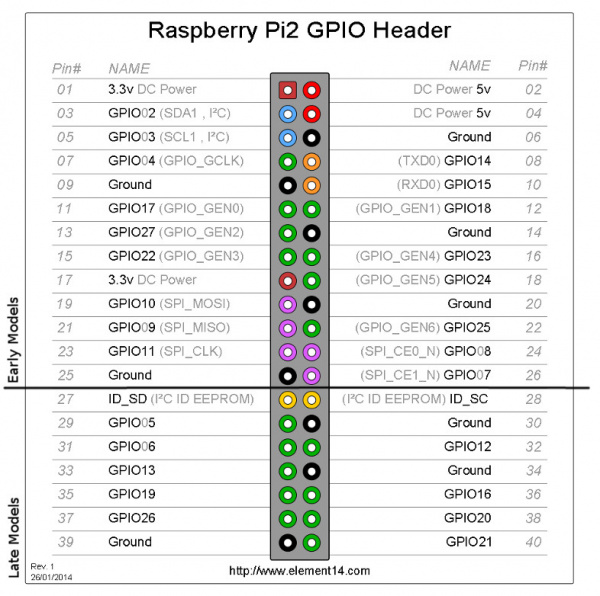
\includegraphics[width=1.0\textwidth]{header_pinout.jpg}\\[0.1in]
In this project we have used the raspberry pi as a camera for taking snapshots from the machine and sending the stream of jpeg images to the website for live monitoring.  
}\\
\section{Polling Code}
{\normalsize Polling is a term used to describe a continuous act of the computer or electronic device checking to verify connections on the computer or device are connected or operating properly.\\[0.1in]
In this project polling was done to fetch the instructions from the simulator model of the database and update the simulator states based on these inputs. The polling is performed once in every 5 secs for updating the states of the simulator running on different threads for each robot as well as for each vessel. \\[0.1in]
Although python has an inbuilt library that supports polling but here we have developed a poller module from scratch just to ensure flexibility of use and application. 
}
\section{Video Streaming Technology}
{\normalsize For video streaming we have made use of Raspi Camera V2 for quick and easy use along with the Raspberry Pi Zero. HTTP protocol was used for transferring snapshots to the server in JPEG format. This stream of JPEG images was loaded directly into the website for live streaming. \\[0.1in]
Although we also worked on UV4L streaming server to use MJPEG protocol to embed live video feed on the website, it could not be integrated in the final simulator through polling only. 
}
\section{Raspberry Pi Camera and UV4L Streaming server}
{\normalsize The Raspi Camera V2 can be connected to the raspberry pi and has the functionality to shoot, record and take snapshots. With Open CV it can also be used to detect motion sensing and face detection. \\[0.1in]
The UV4L provides the following functionalities :\\
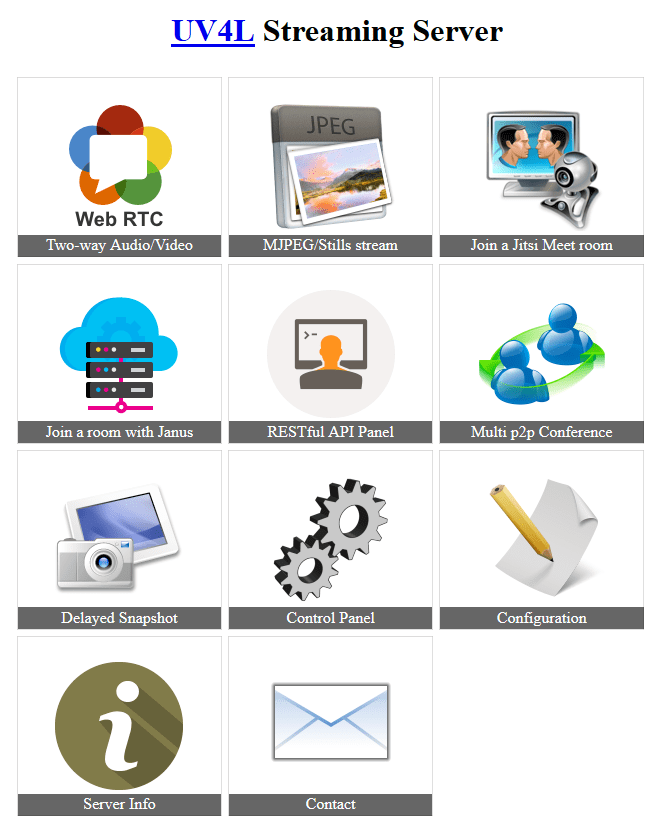
\includegraphics[width=0.8\textwidth]{uv4l_server_main.png}\\[0.1in]
}
\section{Tech Stack}
{\normalsize 
\begin{itemize}
    \item Frameworks : Django, Rasbian
    \item Languages : Python, HTML, CSS and Bootstrap 
    \item Backend database : MySQL
    \item Hardware : Raspberry Pi Zero, Raspicam
\end{itemize}
}




